\documentclass[12pt]{article}

\usepackage{amsmath,amsthm,amssymb,hyperref,fullpage,palatino,bm}

\usepackage{tikz}
\usetikzlibrary{positioning}

\newtheorem{thm}{Theorem}
\newtheorem{cor}{Corollary}
\newtheorem{lem}{Lemma}
\newtheorem{con}[thm]{Conjecture}
\newtheorem{rem}{Remark}
\newtheorem{dfn}{Definition}

\newcommand{\R}{\mathbb{R}}

\newcommand{\x}{\boldsymbol{x}}
\renewcommand{\a}{\boldsymbol{a}}
\renewcommand{\b}{\boldsymbol{b}}
\newcommand{\z}{\boldsymbol{z}}
\newcommand{\X}{\boldsymbol{X}}
\newcommand{\y}{\boldsymbol{y}}
\newcommand{\yh}{\hat{\boldsymbol{y}}}
\newcommand{\w}{\boldsymbol{w}}
\newcommand{\A}{\boldsymbol{A}}
\newcommand{\bdelta}{\boldsymbol{\delta}}

\newcommand{\mse}{\mathrm{MSE}}

\newcommand{\cL}{\mathcal{L}}

\title{Backpropagation for sequential neural networks with densely connected layers}
\author{Pawel Wocjan}

\begin{document}

\maketitle


\begin{abstract}
We introduce neural networks with densely connected layers and describe the backpropagation algorithm for efficiently training these networks.
\end{abstract}

\section{Forward propagation}
We consider a sequential neural netowork consiting of the $L$ densely connected layers of sizes $n^\ell$, where $\ell\in\{0,\ldots,L-1\}$ is used to enumerate the layers.

For $\ell \ge 1$, we denote the weight of the connection from the $k$th neuron in the $(\ell - 1)$th layer to the $j$th neuron in the $\ell$th layer by
\begin{equation}
w^\ell_{jk}
\end{equation}
The diagram below shows two examples. The considered connections are drawn thicker.

\tikzset{
  every neuron/.style={
    circle,
    draw,
    minimum size=1cm
  },
  %neuron missing/.style={
  %  draw=none, 
  %  scale=4,
  %  text height=0.333cm,
  %  execute at begin node=\color{black}$\vdots$
  %},
}

\medskip
\begin{center}
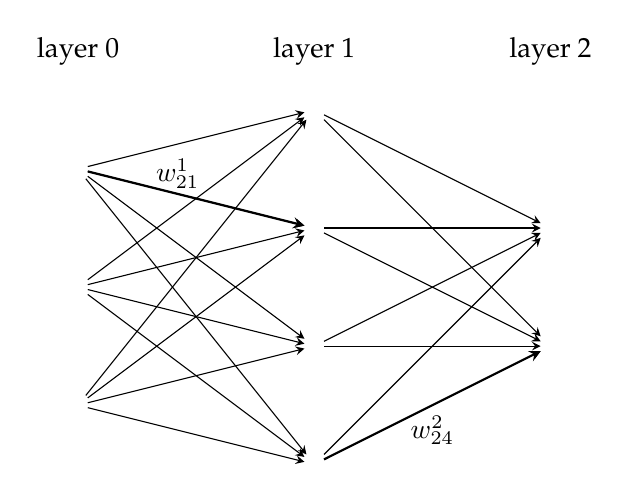
\begin{tikzpicture}[x=1.5cm, y=1.5cm, >=stealth]

\foreach \m/\l [count=\y] in {1,2,3}
  \node [every neuron/.try, neuron \m/.try] (input-\m) at (0,2-\y) {};

\foreach \m [count=\y] in {1,2,3,4}
  \node [every neuron/.try, neuron \m/.try ] (hidden-\m) at (2, 2.5-\y) {};

\foreach \m [count=\y] in {1,2}
  \node [every neuron/.try, neuron \m/.try ] (output-\m) at (4, 1.5-\y) {};

% arrows

%\foreach \l [count=\i] in {1,2,3}
%  \draw [<-] (input-\i) -- ++(-1,0)
%    node [above, midway] {$I_\l$};

%\foreach \l [count=\i] in {1,n}
%  \node [above] at (hidden-\i.north) {$H_\l$};

%\foreach \l [count=\i] in {1,n}
%  \draw [->] (output-\i) -- ++(1,0)
%    node [above, midway] {$O_\l$};

\foreach \i in {1,2,3}
  \foreach \j in {1,2,3,4}
    \draw [->] (input-\i) -- (hidden-\j);

\foreach \i in {1,2,3,4}
  \foreach \j in {1,2}
    \draw [->] (hidden-\i) -- (output-\j);

\foreach \l [count=\x from 0] in {layer 0, layer 1, layer 2}
  \node [align=center] at (\x*2,2) {\l};
  
\draw [->, thick] (hidden-4) -- (output-2) node[midway, below]{$w^2_{24}$};

\draw [->, thick] (input-1) -- (hidden-2) node[midway, above]{\!\!\!\!\!\!\!\!$w^1_{21}$};
\end{tikzpicture}
\end{center}

We use a similar notation for the network's biases and activations. Let
\begin{equation}
b^\ell_j, \quad z^\ell_j, \quad a^\ell_j
\end{equation}
denote the bias, weighted input, and activation of the $j$th neuron in the $\ell$th layer, respectively.



\medskip
\begin{center}
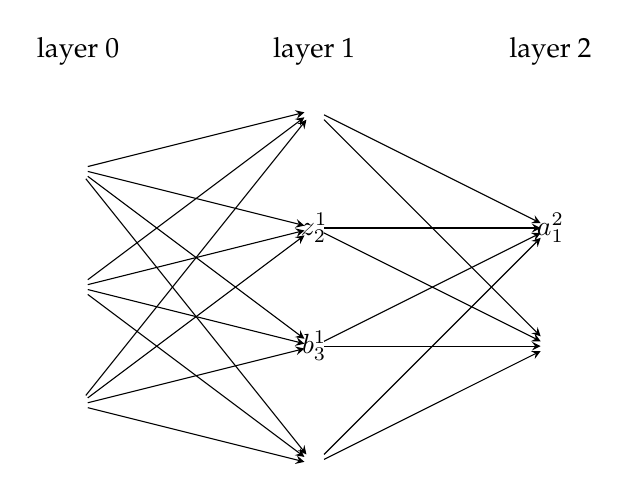
\begin{tikzpicture}[x=1.5cm, y=1.5cm, >=stealth]

\foreach \m/\l [count=\y] in {1,2,3}
  \node [every neuron/.try, neuron \m/.try] (input-\m) at (0,2-\y) {};

\foreach \m [count=\y] in {1,2,3,4}
  \node [every neuron/.try, neuron \m/.try ] (hidden-\m) at (2, 2.5-\y) {};

\foreach \m [count=\y] in {1,2}
  \node [every neuron/.try, neuron \m/.try ] (output-\m) at (4, 1.5-\y) {};

\foreach \i in {1,2,3}
  \foreach \j in {1,2,3,4}
    \draw [->] (input-\i) -- (hidden-\j);

\foreach \i in {1,2,3,4}
  \foreach \j in {1,2}
    \draw [->] (hidden-\i) -- (output-\j);

\foreach \l [count=\x from 0] in {layer 0, layer 1, layer 2}
  \node [align=center] at (\x*2,2) {\l};
  
\node[] at (hidden-3) {$b^1_3$};

\node[] at (hidden-2) {$z^1_2$};

\node[] at (output-1) {$a^2_1$};
\end{tikzpicture}
\end{center}

To keep the discuss genearl, we use $f^{[(\ell)]}$ to denote the activation function of the neurons in the $\ell$th layer. This is because the activation functions for different layers do not always have to be equal.\footnote{We exlude the softmax activation function for now. We only consider activation functions that are applied by each neuron independently. These include sigmoid, tangent hyperbolicus, relu activation functions. We treat the softmax activation function later.}

The forward propagation is described by the following formulas in index notation. We use $k\in\{0,\ldots,n^{[(0)]}-1\}$ to enumerate all neurons the $0$th layer, which is the input layer. For each neuron $k$ of the input layer, we set its activation to
\begin{equation}
  a^{[0]}_k = x_k
\end{equation}
where the value $x_k$ is the $k$th entry of feature vector $\x\in\R^{n^{[0]}}$ that is input the network. (Obviously, the input neurons do not have any weights, biases, or weighted inputs.)

We use $j\in\{0,\ldots,n^\ell-1\}$ to enumerate all neurons of the $\ell$ layer, where $\ell\ge 1$. For each neuron of the layer $\ell$, we have
\begin{align}
z^\ell_j &= \sum_{k=0}^{n^\ell-1} w^\ell_{jk} \cdot a^{\ell-1}_k + b^\ell_j \\
a^\ell_j &= f^\ell(z^\ell_j)
\end{align}
where the sum is taken over all neurons in the $(\ell-1)$th layer. 

To rewrite the above formulas in a matrix form we define a weight matrix
\begin{equation}
W^\ell = \Big( w^\ell_{jk} \Big) \in \R^{n^{\ell-1} \times n^\ell}
\end{equation}
for each layer $\ell$. Similarily, we define the bias vector $\b^\ell\in\R^\ell$ and the activation vector $\a^\ell\in\R^\ell$ for each layer $\ell$.

The forward propagation in  matrix notation is as follows. For the input layer, we set
\begin{equation}
\a^{0} = \x 
\end{equation}
For the $\ell$th layer, where $\ell\ge 1$, we have
\begin{align}
\z^\ell &= W^\ell \a^{\ell-1} + \b^\ell \\
\a^\ell &= f^\ell (\z^\ell)
\end{align}

\section{Loss function}
The goal of backpropagation is to compute the partial derivatives
\begin{equation}
{\partial \cL \over \partial w^\ell_{jk}}  \quad\mbox{and} \quad {\partial \cL \over \partial b^\ell_j}
\end{equation}
with respect to any weight and bias of the network. We need these partial derivatives to be able to apply stochastic gradient descent.

Let $\x\in\R^{n^{0}}$ be a feature vector and $\y\in\R^{n^{L-1}}$ its corresponding target vector.\footnote{For instance, this could be the the one-hot-encoding vector.} 
For obvious reasons, we need to assume that the loss function $\cL$ is a function of the target vector $\y$ and the output of the neural network $\a^{L-1}$ that is produced when $\x$ isthe input. Also, we assume that the loss for a mini-batch is given by the mean of the losses for the individual examples of the mini-batch.

\section{Backpropagation}

Assume that a friendly demon sits in the $j$th neuron in layer $\ell$. As the weighted input $\z^\ell_j$ is formed, the demon messes with the neuron's operation. It adds a little change $\Delta \z^\ell_j$ to $\z^\ell_j$, so the neuron outputs $f^\ell(\z^\ell_j + \Delta \z^\ell_j)$ instead of $f^\ell(\z^{\ell}_j)$. This changes is propagated through the subsequent layers, finally causing the loss to change by an amount
\begin{equation}
{\partial \cL \over \partial z^\ell_j} \cdot \Delta z^\ell_j.
\end{equation}

This demon is good, and it is trying to decrease the loss, that is, to find a $\Delta z^\ell_j$ that makes the loss smaller. 
\begin{itemize}
\item Suppose the partial derivative ${\partial \cL / \partial z^\ell_j}$ is a large value (either positive or negative). Then the demon can decrease the lost substantially by choosing $\Delta z_j^\ell$ to have the opposite sign to ${\partial \cL / \partial z^\ell_j}$.
\item In contrast, suppose that the partial derivative ${\partial \cL / \partial z^\ell_j}$ is close to zero. Then the demon cannot decrease the loss much by perturbing the weighted input $z^\ell_j$. So far the helpful demon can tell, the neuron is already pretty near optimal. So there is a heuristic sense in which the partial derivative ${\partial \cL / \partial z^\ell_j}$ is a measure for the error in the neuron.
\end{itemize}

We define the delta (error) $\delta^\ell_j$ of the $j$th neuron in the $\ell$th layer by
\begin{equation}
\delta^\ell_j = {\partial \cL \over \partial z^\ell_j}.
\end{equation}
We also define $\bdelta^\ell$ the vector of all errors associated with layer $\ell$ by
\begin{equation}
\bdelta^\ell = \nabla_{\z^\ell} \cL.
\end{equation}

We will see backpropagation gives us an efficient way of calculating $\bdelta^\ell$ for every layer. 

\subsection{Pawel's derivation}

We want to show that 
\begin{equation}
\bdelta^{\ell-1} = (W^{\ell})^T \bdelta^\ell \circ g^{\ell-1}(z^{\ell-1})
\end{equation}
where $\circ$ denotes the Hadamard product and $g^{\ell-1}$ denotes the derivative of $f^{\ell-1}$. Note that $g^{\ell-1}$ is applied elementwise.

First, we have
\begin{align}
{\partial \cL \over \partial a^{\ell-1}_k} 
&=
\sum_j {\partial \cL \over \partial z^\ell_j} \cdot {\partial z^\ell_j \over \partial a^{\ell-1}_k} \\
&=
\sum_j {\delta^\ell_j} \cdot w^\ell_{jk}
\end{align}
and in matrix notation
\begin{align}
\nabla_{\a^{\ell-1}} \cL 
&=
(W^\ell)^T \cdot \nabla_{\z^\ell} \cL \\
&= 
(W^\ell)^T \cdot \bdelta^\ell.
\end{align}
Second, we have 
\begin{align}
{\partial L \over \partial z^{\ell-1}_k} = {\partial \cL \over \partial a^{\ell-1}_k} \cdot {\partial a^{\ell-1}_k \over \partial z^{\ell-1}_k}
\end{align}
and in matrix notation
\begin{equation}
\bdelta^{\ell-1} = \nabla_{\a^{\ell-1}} \cL \circ g^{\ell-1}(\z^{\ell-1})
\end{equation}



\newpage

\subsection{An equation for the delta in the output layer}

The components of $\bdelta^{L-1}$ are given by
\begin{align}
\delta^{L-1}_j 
&= 
{\partial \cL \over \partial a^{L-1}_j} \cdot {\partial a^{L-1}_j \over \partial z^{L-1}_j} \\
&= 
{\partial \cL \over \partial a^{L-1}_j} \cdot g^{L-1}(z^{L-1}_j),
\end{align}
where $g^{L-1}$ denotes the derivative of the activation function $f^{L-1}$.

Note that everything is easily computed. In particular, we compute the weighted input $z^{L-1}_j$ during forward propagation, and it's only a small additional cost to compute $g^{L-1}(z^\ell_j)$.
The exact form of ${\partial \cL / \partial a^{L-1}_j}$ depends on the particular loss function used. However, since the loss function is known, it should be easy to compute ${\partial \cL / \partial a^{L-1}_j}$.  

The above equation is in index notation. However, it is easy to rewrite the equation in matrix form as follows
\begin{equation}
\bdelta^{L-1} = \nabla_{\a^{L-1}} \cL \circ g(\z^{L-1}),
\end{equation}
where $\nabla_{\a^{L-1}} \cL$ is defined to the vector whose entries are the partial derivatives ${\partial \cL / \partial a^{L-1}_j}$
and $\circ$ denotes the Hadamard product\footnote{The Hadamard product (also called Schur product) is the entrywise product.} of two vectors.

\subsection{An equation for the delta in terms of the successor's delta}

\end{document}